\documentclass[11pt]{article}


\usepackage[a4paper, total={6in, 8in}]{geometry}
\usepackage{graphicx}
\usepackage{multicol}
\usepackage{multirow}

\title{July2023 CSE300 Week9 Online Evaluation}
\author{2005089}
\date{\today}

\begin{document}

\maketitle
\tableofcontents

\pagebreak 

\section{RISC Architecture}
  \begin{figure}[h]
      \centering
      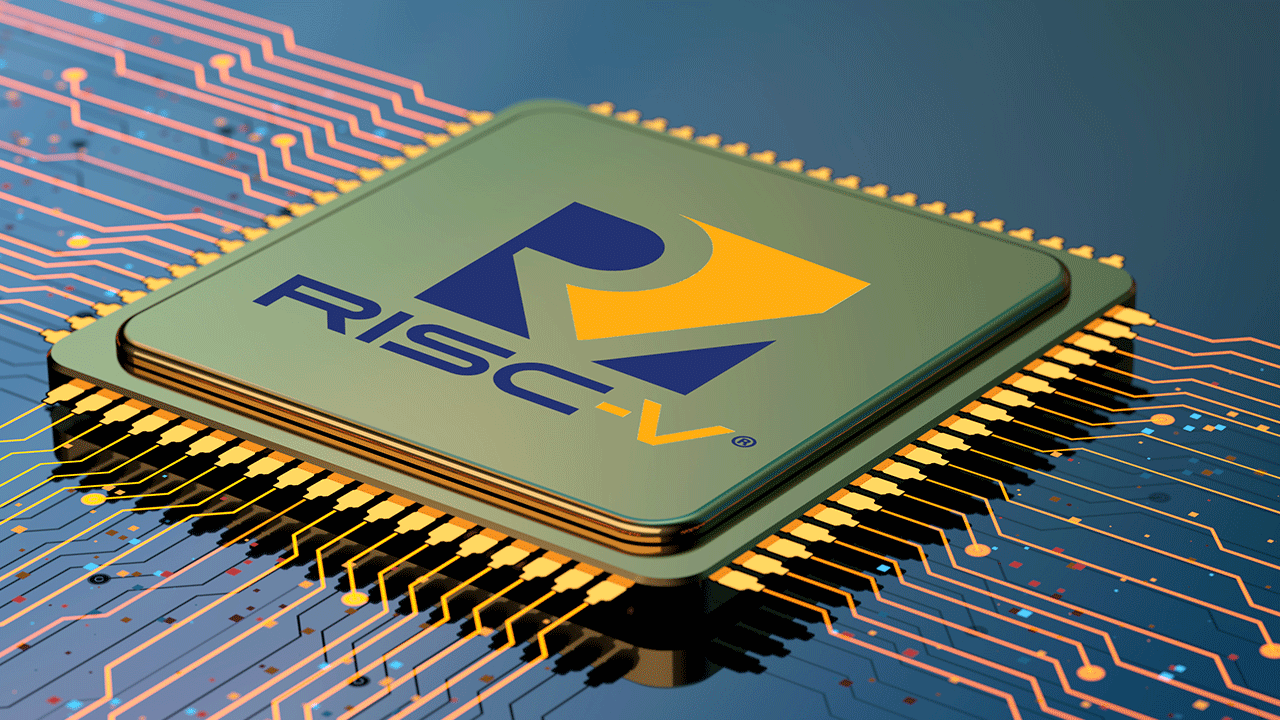
\includegraphics[scale = 0.3]{Images/risc.png}
      \caption{RISC Architecture}
      \label{fig:enter-label}
  \end{figure}

  \section{Tables in \LaTeX}

  \begin{table}[h]
      \centering
      \begin{tabular}{|c|c|c|c|}
           \hline

           \multirow{10}{*}{numeric literals} & \multirow{5}{*}{integers} & in decimal & 8743 \\
           \cline{3-4}
           & & \multirow{2}{*}{in octal} &  07464 \\ 
           \cline{4-4}

           & & & 0D103 \\ 
           \cline {3-4}

           & & \multirow{2}{*}{in hexadecimal} & 0x5A0FF  \\
           \cline{4-4}

           & &  & 0xE0F2 \\
           \cline{2-4}

           & \multirow{5}{*}{fractionals} & \multirow{5}{*}{in decimal} & 140.58 \\
           \cline{4-4}

           & & & 8.04e7 \\
           \cline{4-4}

           & & & 0.347E+12 \\
           \cline{4-4}

           & & & 5.47E-12 \\
           \cline{4-4}

           & & & 47e22 \\
           \hline
      
      
      
      
      
      
      \end{tabular}
      \caption{A table in \LaTeX}
      \label{tab:my_label}
  \end{table}

  \parindent 10mm {Table 1 shows a table that contains cells spanning multiple columns and multiple rows. \cite{random}}


\section{Writing Equations in Latex}

\begin{equation}
    L_{split} = \frac{1}{2} [\ \frac{G_{L}^2}{H_{L} + \lambda} + \frac{G_{R}^2}{H_{R} + \lambda} - \frac{(G_{L}+G_{H})^2}{H_{L} + H_{R} + \lambda} ] - \gamma
\end{equation}


\parindent 10mm {Equation 1 has been displayed above. \cite{greedy}}

\section*{Untitled Section}
{You need to display this section in your output PDF file. This section contains information
that may help you prepare the bibliography section. By the way, this section \textbf{will not
show up} in the table of contents.
}

\begin{enumerate}
    \item \textbf{Citation about the Greedy Forest Article}
    \begin{itemize}
        \item \textbf{Authors: }T. Zhang, R. Johnson 
         \item \textbf{Title: }Learning nonlinear functions using regularized greedy forest
          \item \textbf{Year: }2014
           \item \textbf{Journal: }IEEE Transactions on Pattern Analysis and Machine Intelligence
        
    \end{itemize}
    \item \textbf{Citation about the Random Forest Article}
    \begin{itemize}
        \item \textbf{Author: }L. Breiman
         \item \textbf{Title: }Random Forests
          
           \item \textbf{Journal: } Machine Learning
           \item \textbf{Year: }2001
        
    \end{itemize}
    
     
\end{enumerate}


  \bibliographystyle{abbrv}
   \bibliography{ref}
  

\end{document}
